\documentclass[11pt,a4paper]{report}
\usepackage[utf8]{inputenc}
\usepackage[frenchb]{babel}
%\usepackage{baskervald}
\usepackage{gfsartemisia}
%\usepackage{palatino}
%\usepackage{libertine}
\usepackage[T1]{fontenc}
\usepackage{textcomp} % Pour les symboles spéciaux
\usepackage{listings} % Pour l'ajout de code source
\usepackage{graphicx} % Pour l'ajout des images
\usepackage{titlesec} % Pour ne plus avoir le mot chapitre
\usepackage{lettrine} % Pour l'usage des lettrines

% marge à la Beaufils
\usepackage{geometry}
\geometry{a4paper,top=1.5cm,bottom=1.5cm,right=1.5cm,left=1.5cm}

% Interligne pour le sommaire
%{\setlength{\baselineskip}{1.9\baselineskip}\tableofcontents\par}

% Marge pour la reliure
\addtolength{\hoffset}{+0.5cm}

% Style de page personalisé%{{{
\usepackage{fancyhdr}
\pagestyle{fancy} % Ceci permet d’avoir les noms de chapitre et de section % en minuscules
\renewcommand{\chaptermark}[1]{\markboth{#1}{}}
\renewcommand{\sectionmark}[1]{\markright{\thesection\ #1}}
\fancyhf{}	% supprime les en-têtes et pieds
\fancyhead[LE,RO]{\bfseries\thepage}% Left Even, Right Odd
\fancyhead[LO]{\bfseries\rightmark} % Left Odd
\fancyhead[RE]{\bfseries\leftmark} % Right Even
\renewcommand{\headrulewidth}{1pt}% filet en haut de page
\addtolength{\headheight}{14pt}	% espace pour le filet
\renewcommand{\footrulewidth}{0pt} % pas de filet en bas
\fancypagestyle{plain}{ % pages de tetes de chapitre
\fancyhead{}	% supprime l’entete
\renewcommand{\headrulewidth}{0pt} % et le filet
}%}}}

%Couverture%{{{

\title
{
	\normalsize{IUT A Lille 1 - Villneuve-d'Ascq\\
	2012-2013}\\
	\vspace{15mm}
  \Huge{Barcraft
    \vspace{15mm}}
}
\author{
\bsc{Stechele} Julien\\
\bsc{Vanuxem} Yannick\\
\bsc{Serir} Jean-francois\\
	\vspace{30mm}
}
%}}}

\begin{document}%{{{

\maketitle
\tableofcontents
\newpage

\chapter{Remerciements}%{{{
\label{cha:remerciements}

\lettrine{N}{ous} tenons tout d'abord à remercier :

\begin{itemize}

\item \bsc{Me.~Belot}, professeur de technique d'expression pour nous
avoir enseigné la prise de parole en public ainsi que les bonnes
pratiques d'un déroulement de projet.

\item \bsc{M.~Beaufils}, Maître de conférence et responsable de la
formation \emph{Développement \& Administration de site Internet \&
intranet}(DA2I) pour cette dernière année de licence captivante.

\item \bsc{M.~Mathieu}, Vice-président délégué technologie de
l'information et de la communication et professeur de base de données et
web pour l'aide et les conseils apportés lors de la préparation de
l'événement.

\item \bsc{M.~Trique}, administrateur système de l' \og l'Institut
Universitaire de Technologie \fg{} (IUT A) sans qui ce projet n'aurait pas
eu lieu. Il nous a permis d'acquérir une certaine crédibilité auprès des
responsables du réseau de la cité scientifique.

\item \bsc{M.~Digeo}, président de l' \og Association des Étudiants en
Informatique \fg{} (AEI) et \bsc{M~Dewarumez}, leur trésorier, pour
leurs conseils sur l'organisation et leur soutien tout au long du
projet.

\item \bsc{M.~Bros}, responsable de la \og Maison Des Étudiants \fg{}
(MDE) ainsi que \bsc{M.~Ferla}, président de l'\og Association des aMis
de l'Université de Lille 1 \fg{} (AMUL) pour leurs disponibilités et
leurs aides.

\end{itemize}


% chapter remerciements (end)%}}}
\chapter{Les prémices du projet}%{{{
\label{cha:les_pr_mices_du_projet}

\section{L'objectif du projet de communication}%{{{
\label{sec:l_objectif_du_projet_de_communication}

Les principaux objectifs du projet de communication sont :

\begin{enumerate}

\item Promouvoir la formation au travers d'activités tantôt éducatives
tantôt lucrative ;

\item S'ouvrir au monde extérieur en montrant que des projets en dehors
de l'informatique sont menées au sein de la licence professionnelle ;

\item Faire face a des responsabilités et à la pression que celle-ci
peut entrainer ;

\item Mener de bout en bout l'élaboration d'un projet, qui plus est en
groupe.

\end{enumerate}

% section l_objectif_du_projet_de_communication (end)%}}}
\section{L'idée principale}
\label{sec:l_idee_principale}

\lettrine{A}{yant} une passion commune autour de l'eSport\, \footnote{Ce
mot est expliqué en section \ref{sec:le_sport_electronique_esport_} à la
page \pageref{sec:le_sport_electronique_esport_}.} et des jeux vidéos en
général, nous cherchions un projet ambitieux et original pour promouvoir
la formation. Nous ne voulions pas d'un projet maintes et maintes fois
réalisé et finalement peu motivant qui aurait reflété en nous
l'obligation de faire plutôt que l'envie de faire. Ayant suivi avec
attention la montée en puissance d'un nouveau phénomène qu'est le
Barcraft\, \footnote{Expliqué dans la même partie à la page
\pageref{sec:barcraft}.} nous nous sommes mis en tête de présenter cette
idée et de la défendre.

% section l_idee_principale (end)
\section{Les jeux considérés}%{{{
\label{sec:les_jeux_consideres}

\lettrine{L}{ors} de nos réunions nous avons eu plusieurs idées de jeux
à présenter pendant la soirée. En effet, nous nous sommes dit que
Starcraft (nous expliquons un peu plus loin ce que c'est) était
peut-être un segment trop étroit pour attirer du monde et qu'il valait
mieux présenter plusieurs jeux en proposant des plages horaires pour
ceux-ci. Nous allons voir plus loin que cette idée ne fut pas retenue au
final.

\begin{description}

\item[Starcraft - Brood War :] Celui-ci devait être présenté pour
montrer les différences de graphismes et de gameplay de la franchise au
fil des années mais il n'y avait qu'une personne du groupe qui possédait
le jeu -- qui est en plus décomposé en un jeu + une extension -- ce qui
fait que les autres devaient l'acquérir pour la soirée. De plus, \og
Brood War \fg{} par son graphisme 2D aurait surement fait fuir le public. 
Celui-ci est présenté dans la section
\emph{Présentation}.

\item[Starcraft II :] Le jeu principal auquel tous les membres du groupe
jouent et connaissent bien. Celui-ci est décomposé en deux jeux distincts.
La partie la plus intéressante étant le jeu en ligne bien évidemment.
L'extension \og Heart of the Swarm \fg{} étant sortie la veille de la
soirée il a fallu nous empresser de l'acheter pour pouvoir y jouer et
ainsi montrer les nouvelles unités du jeu. Ce jeux est le premier auquel
nous ayons pensé tout simplement parce que c'est celui-ci qui a
démocratisé le concept de Barcraft.

\item[League of Legends :] C'est un jeu très connu qui aurait attiré
beaucoup de monde car plus accessible au premier abord. Seulement, il
n'y a qu'une personne du groupe qui y joue. Il fallait aussi trouver des
joueurs et un commentateurs spécifiquement pour celui-ci. \emph{LoL} est en plus
un jeu qui se joue en équipe de cinq ce qui complexifie grandement la
recherche d'intervenants.

\item[Retro-gaming :] On voulait proposer d'autres jeux de stratégie
d'anthologie à côté des matchs commentés mais cela aurait dénaturé le
projet pour finir en soirée jeux vidéo, ce qui n'a jamais été notre
intention. De plus, il aurait fallu encadrer un nombre conséquent de
matériel durant la soirée ce qui aurait été dur à gérer à trois
personnes.

\item[Jeu de plateau :] Nous avons pensé à nous procurer des jeux de
plateaux. En effet, l'association \emph{Dés à la Carte} organise ce
genre d'événement assez régulièrement. Nous avons décidé assez vite de
ne pas retenir cette idée car cela aurait causé trop de dispersions dans
la soirée et le concept de Barcraft n'aurait plus eu de sens.

\end{description}

Au final nous sommes revenus sur nos idées. Nous avons décidé
de ne présenter que Starcraft II qui est le jeu que nous connaissons le
plus. Cependant certains des jeux ont été encore proposés un mois avant
la date butoire, c'est pourquoi ceux-ci sont présentés dans ce rapport.

% section les_jeux_consideres (end)%}}}
\section{La soumission de l'idée}%{{{
\label{sec:la_soumission_de_l_idee}

\lettrine{N}{ous} avons cherché à démystifier la pratique des jeux vidéo, 
soumise malgré elle à un certain nombre d'idées reçues et de
préjugés. Il fallait mettre en avant l'aspect stratégique des jeux
choisis et la professionnalisation de ceux-ci qui est en pleine expansion. 
Cependant nous nous sommes heurtés aux règles bien définies du projet de
communication qui devait le plus possible se dérouler loin de
l'informatique et du monde numérique, autant dire que nous ne partions
pas gagnants même si nous étions très motivés et déterminés à convaincre
nos enseignants. Il y a eu des moments d'incertitudes mais nous nous
sommes efforcés à nous motiver les uns les autres. Nous avons dû
défendre à plusieurs reprises nos idées comparées aux autres projets ce
qui nous a demandé une plus grande clarté sur nos intentions.

% section la_soumission_de_l_idee (end)%}}}
\section{Projet accepté}%{{{
\label{sec:projet_accepte}

\lettrine{N}{otre} projet a mis plus de temps que les autres à être
validé. Celui-ci devait être soumis à deux personnes. Nous nous sommes
retrouvé pendant un laps de temps (2 semaines) sans savoir si notre
projet était validé ou non. Nous étions inquiets parce que s'il n'était
pas accepté, cela nous aurait mis grandement en retard pour 
en trouver un nouveau mais également mettre ce nouveau projet sur pied. Nous
avions pensé à plusieurs solutions de remplacement mais celles-ci ne nous
motivait pas autant voir pas du tout comparé à notre idée principale.

Nous avions pensé à :

\begin{description}

\item[Tournois de tennis de table :] Deux membres du groupe en ont fait en
club et aimennt ce sport cependant il est très difficile de se procurer du
matériel pour tout un tournoi ;

\item[Post-it war :] le concept est de proposer aux gens des différents
bâtiments de Lille 1 de faire de grands dessins sur les baies vitrées
avec des post-it de couleurs. Les dessins aurait été soumis à des juges
qui aurait décerné la meilleur \oe{}uvre.  Pour l'anecdote, cette idée à
été réalité à la fin de cette année par l'AEI.

\end{description}

Heureusement pour nous, nous n'avons pas eu besoin d'y réfléchir
d'avantage et nous avons du nous mettre au travail pour réaliser notre
projet.

% section projet_accepte (end)%}}}


% chapter les_pr_mices_du_projet (end)%}}}
\chapter{Présentation}%{{{
\label{cha:presentation}

\subsection{Jeux de stratégie en temps réel}%{{{
\label{sub:jeux_de_strategie_en_temps_reel}

\lettrine{U}{ne} très bonne définition de ce qu'est le jeux de stratégie en
temps réel est consultable sur wikipédia :

  Le jeu de stratégie en temps réel (STR, ou RTS pour la
  dénomination du genre en anglais : real-time strategy) est un type de
  jeu de stratégie particulier qui notamment et par opposition au jeu de
  stratégie au tour par tour n’utilise pas un découpage arbitraire du
  temps [...]

  Dans le tour par tour, donc, l'issue d’une confrontation est résolue par
  étapes, un combat en succédant un autre, de manière à laisser à chaque
  joueur le temps de réfléchir sur la prochaine étape. Une confrontation
  est alors résolue par combats successifs et isolés.

  Mais le problème qui se pose lorsqu'on veut simuler des affrontements
  réalistes est qu’en général, les unités n’attendent pas que ce soit leur
  tour pour attaquer et gérer l'affrontement de plusieurs unités en même
  temps et de façon réaliste relève du domaine de l'impossible pour l'être
  humain, jusqu'à l'invention des processeurs. Ceux-ci, programmés de
  manière à simuler un affrontement peuvent désormais gérer le déplacement
  de plusieurs unités simultanément et résoudre les combats de façon
  simultanée et rigoureuse dans le cadre d’un jeu vidéo.

% subsection jeux_de_strategie_en_temps_reel (end)%}}}
\subsection{Le sport éléctronique (eSport)}%{{{
\label{sub:le_sport_electronique_esport_}

\lettrine{L}{’eSport} (ou sport électronique) est un terme désignant le
système compétitif mis en place dans le domaine des jeux-vidéo
multi-joueurs.  A la manière des sports physiques, l'eSport s’est
professionnalisé à partir de la fin des années 90. Il existe donc des
équipes de joueurs professionnels pouvant posséder un entraineur, un
manager ou encore des sponsors. Par exemple, la somme totale des
récompenses mises en jeu pour Starcraft 2 sur toute l’année 2011 atteint
2,5 millions d’euros.  Mais l'eSport en est encore à ses débuts,
l'absence d'une autorité « eSportive » laisse subsister des délais de
paiement ainsi que des non payés.

% subsection le_sport_electronique_esport_ (end)%}}}
\subsection{La licence Starcraft}%{{{
\label{sub:la_licence_starcraft}

\subsubsection{Starcraft \& Starcraft : Brood War}%{{{
\label{ssub:starcraft_&_starcraft_brood_war}

\lettrine{S}{tarcraft} est un jeu vidéo de stratégie en temps réel (STR) développé
par Blizzard Entertainment. Le premier opus est sorti en Europe le 31
mars 1998 sur PC. Il s'inscrit dans la lignée des jeux de stratégie de
Blizzard maintenant très populaire auprès des amateurs du genre. Avec
plus de 11 millions de copies vendues dans le monde, il est un des
jeux vidéo sur PC les mieux vendus et reste à ce jour le jeu de
stratégie en temps réel le plus vendu de tout les temps.

(image)

% subsubsection starcraft_&_starcraft_brood_war (end)%}}}
\subsubsection{Starcraft 2 : Wings of Liberty}%{{{
\label{ssub:starcraft_2_wings_of_liberty}

\lettrine{C}{elui}-ci sort dans le monde après 12 ans d'attente
interminable le 27 juillet 2010. Blizzard ayant fait le choix marketing
de faire trois campagnes distinctes, il y aura deux extensions de
prevues ce qui à fait polémique à l'époque. Avec le deuxième opus,
blizzard à fait le pari de démocratisé le jeux de stratégie en temps
réel en rendant WoL plus facile d'accès comparées a Brood War qui lui
requiérait beaucoup d'APM (nbp). Pari reussi puisqu'il connait
rapidement un important succès commercial avec plus de 4,5 millions de
copies vendues 6 mois après la sortie du jeu.

(image)

% subsubsection starcraft_2_wings_of_liberty (end)%}}}
\subsubsection{Starcraft 2 : Heart of the Swarm}%{{{
\label{ssub:starcraft_2_heart_of_the_swarm}

\lettrine{H}{eart} of the Swarm est la première des deux extensions
prévu du jeux Starcraft 2. Elle constitue la suite du premier chapitre
Wings of Liberty. La date de sortie officielle est le 12 mars 2013 soit
deux ans et demi après le premier opus.  Aucune statistique de vente n'a
encore été publiée par blizzard actuellement.

% subsubsection starcraft_2_heart_of_the_swarm (end)%}}}

% subsection la_licence_starcraft (end)%}}}
\subsection{League of Legends}%{{{
\label{sub:league_of_legends}

League of Legends est un jeu de stratégie en équipe de type
MOBA(Multiplayer Online Battle Arena). Au début d'une partie, quelque
soit le mode de jeu, chaque joueur choisit un héros qu'il va représenter
sur le champ de bataille. Les aspects coordination et travaille d'équipe
sont très important pour le déroulement de la partie. Tout un panel de
stratégie de jeu sont à notre disposition afin de prendre l'avantage sur
l'équipe adverse, le but étant de détruire la base adverse afin de
gagner la partie.

% subsection league_of_legends (end)%}}}
\subsection{Barcraft}%{{{
\label{sub:barcraft}

\lettrine{C}{omme} sous nom l'indique, il s'agit d'organiser une soirée
autour du jeu Starcraft dans l'ambiance d'un bar.	Pour cela, nous
faisons appelle à des intervenants extérieurs. Afin d'ouvrir un maximum
de spectacle, nous avons demander à des joueurs professionnels ainsi que
des commentateurs professionnels de participer à l'événement.  La soirée
se déroule sous la forme de matchs commentés. Pour une bonne interaction
avec le public, les matchs sont vidéo projetés sur un écran géant. Au
cour de la soirée les joueurs du public pourront prendre place et jouer
contre nos joueurs professionnels.

% subsection barcraft (end)%}}}


% chapter presentation (end)%}}}
\chapter{Organisation}%{{{
\label{cha:organisation}


\section{Technique}%{{{
\label{sec:technique}

Afin que la soirée se déroule sans encombre il nous faut une connexion
internet avec certains ports pour certains protocoles débloqués, et ce
n'est pas une mince affaire. Tout d'abord nous avons demander l'avis de
monsieur Mathieu et la procédure à suivre dans ce genre de cas.  Au fil
des échanges nous avons donc fixé le lieu, le périmètre, la date, la
durée, le nombre d'ordinateur et quelques autres points techniques.
Dans un premier temps, les tests se font dans notre salle de tp
habituelle et notre intermédiaire pour les détails techniques est
monsieur Eric Triquet.  Les premiers tests se font sur un seule machine,
un ordinateur portable personnel, on utilise un adresse ip public et les
tests sont plutôt satisfaisants.  Le déploiement vers la maison des
étudiants pose problème. Le responsable sécurité ne veut pas ouvrir
quatres adresses ip public vers des ordinateurs personnels, ce qui veut
dire que nous devons penser à autre chose.  La solution à ce problème a
été trouver en allant directement au CRI avec monsier Triquet afin de
s'expliquer sur les besoins de la soirée.  Nous avons donc établi un
terrain d'entente, la solution est d'utiliser un VLAN, c'est un réseau
indépendant et isolé du reste du réseau et permet de garder un contrôle
sur les données transmises lors de notre soirée.  Les tests en salle tp
se sont montrés concluants, et le déploiement sur la maison des
étudiants n'a pas été long.  Les tests finaux sur site se sont montrés
également concluant.
Pour que la soirée se déroule dans les règles de l'art, il nous fallait
du materiel spécifique. En effet, comme expliqué dans la section
barcraft (link) des ordinateurs, une connexion à internet et un
vidéo-projecteur sont requis (et de la bière si possible) pour prétendre
organiser ce type d'evenement.

% section technique (end)%}}}
\section{Materiel}%{{{
\label{sec:materiel}

  Starcraft 2 est un jeu assez reçent comme nous l'avons vu dans la
partie (link) ce qu'il fait qu'il requiert des machines puissantes pour jouer
dans bonnes conditions. Nous avons tout d'abord cherché à emprunté des
machines auprès de l'AEI mais celle-ci - à part pour faire tourner brood
war - sont mauvaises étant donnée qu'elle ne contienne qu'un chipset
graphique (explication). Par la suite nous avons discuté avec les
intervenants pour que ceux-ci ramènent leurs configurations. Ça nous
aurait permis de nous soulager un peu mais aussi d'améliorer la qualité
de jeux du joueur professionnel. Il est connu que l'on joue mieux sur sa
propre machine - avec laquel on à l'habitude - plutôt que la machine d'un
autre.

Les autres materiaux dont nous avions besoin comme le videoprojecteur,
les micros, la connectique et les tables/chaises était disponible directement à
la maison des étudiants ce qui nous a grandement facilité la tâche.

Pour ce qui est de l'isolation des joueurs, nous avons décidé un peu à
la dernière minute qu'un casque de chantier et des écouteurs
intra-oriculaires suffirait. C'est ce qui est utilisé la pluspart du
temps sauf pour les gros évenements qui eux construisent des "box
insonorisées". Étant donnée que notre projet n'est pas de la même
envergure nous nous en sommes passé bien évidemment.

% section materiel (end)%}}}
\section{Salle et bar}%{{{
\label{sec:salle_et_bar}

Nous cherchions un local qui aurait le maximum de materiel dont nous
avions besoin pour la soirée pour plus de facilité. Nous avons tout
dabord cherché a l'interieur du campus de lille avant de vouloir trouvé
un commerce qui nous aurait demandé beaucoup plus d'éffort d'un point de
vue recherche (le concept étant peu connu du grand public sa aurait été
très difficile).

Ayant participé a certaines soirées étudiantes qui se déroule le jeudi
soir a la maison des étudiants (MDE), nous avons remarqué que celle-ci
était disponible assez facilement, gratuitement et avec du materiel
approprié. En effet, les thématiques proposées par la MDE sont très
diverses. Elle peut aussi bien faire office de salle de reunion que de
concert ou même de soirée cinéma.

Cependant, pour avoir le droit d'organiser quelquechose dans celle-ci il
faut appartenir à une association étudiante connu du campus. Aucun
membre du groupe étant licencé dans ce genre d'initiative nous étions un
peu inquiet. Après s'être renseigné a differents endroits, il faut
simplement se rapprocher d'une association pour qu'elle puisse se porte
garant de l'évenement.

La nécéssité d'avoir une association derrière nous est obligatoire pour
l'obtention d'une extension d'assurance pour les biens et les personnes
au cas ou un problème majeur surviendrait lors de la soirée.

L'AMUL est l'association qui prend en charge le bar de la maison des
étudiants.  Pour pouvoir assurer une permanence pour notre soirée, nous
avons du contacter le président de cette association afin de demander
son accord.  Un échange par mail est alors effectué, pour conclure avec
un rendez-vous pour définir nos attentes concrètes et si elles sont
réalisables. Suite à cet entretien il a été convenu qu'une permanence
aura lieu de 18h à 22h.

% section salle_et_bar (end)%}}}
\section{Partenariats et sponsors}%{{{
\label{sec:partenariats_et_sponsors}

- Demande de financement du projet auprès de la FSDIE (Fonds de solidarité
et de Développement des Initiatives Etudiantes)

Nous nous sommes tout dabord rendu au batiment A3 pour récupéré un
dossier de demande de financement pour les projets des étudiants. Ce
dossier requierait un certain nombre de pièces justificatives comme le
planning de déroulement de la soirée, le montant envisagé, le potentiel
nombre de participant ainsi qu'au final un entretiens avec les membres
du groupe face à un jury pour prétendre avoir cette aide. Nous avons
abandonnée cette possibilité car nous ne savions pas si le projet était
possible vis à vis de la connexion à internet requise.

%TODO
- collaboration avec l'aei

Nous avons choisi de traiter avec l'AEI (association des étudiants
en informatique) qui sont des habituées de ce genre de soirée à
thématique *geek* et emprunteur historique de la maison des étudiants.
Leur principal local ce situe dans le batiment M5 au milieu de la
cité scientifique ou sont concentré la pluspart des informaticiens de
lille1.
Nous avons donc exposé notre projet avec ceux-ci

- demande de financement auprès de Micromania (v2)

Une demande de financement à été faite auprès du célèbre magasin de
jeux-vidéo Micromania qui nous a vallu un refus cathégorique. Cette
enseigne ne sponsorisant pas d'évenement par soucis
budgétaire.

%TODO
- demande de sponsor Materiel.net (lomme)

Nous avons également contacté Materiel.net afin de savoir s'ils pouvaient nous prêter,
louer du matériel ou encore sponsoriser la soirée mais ils n'étaient pas intéressés.

%TODO
- envoie d'un mail au service communication sans reponse

N'ayant trouvé aucun moyen de financement pour permettre aux
intervenants et nous même de nous restaurer lors de l'évènement, nous
n'avions pas d'autre choix que de répartir les coûts entre membre du
projet. C'est à ce moment la que le responsable de la formation DA2I
proposa de débloqué les fonds allouées à la licence pour permettre de
financer les évènements des étudiants. Ce fut une aubaine pour nous.

Nous avons tout dabord pensé à acheter nous même les aliments pour
ensuite ce faire rembourser avec cette somme mais cela posait des
problèmes logistiques. Une autre idée à donc été proposé : commander des
plateaux repas (qui est un service proposé par l'iut). Il nous a donc
été demandé de réunir des informations auprès des intervenants de la
soirée, comme leur nom, prénom, adresse, fonction pour que cette demande
aboutisse.

% section partenariats_et_sponsors (end)%}}}
\section{Intervenants}%{{{
\label{sec:intervenants}

\subsection{Le rôle des intervenants}%{{{
\label{sub:le_role_des_intervenants}

Nous souhaitions invité des personnes exterieures pour le projet à
différente fins. Il nous fallait un ou des commentateurs ainsi que des
joueurs qui sachant que leurs parties allait être commenté devait faire
le show pour le public. Ceux-ci, pour engrangé du monde, devait être
connu de la scène française.

% subsection le_role_des_intervenants (end)%}}}
\subsection{Alexandre "Makoz" Chilling}%{{{
\label{sub:alexandre_makoz_chilling}

Un des membres du groupe qui, connaissant bien la scène française autour
de starcraft 2, s'est occupé de contacter des intervenants.  Celui-ci,
appréciant Alexandre "maKoZ" Chilling la contacté en premier.  maKoz qui
était (au moment de la demande) manager de *spart legion*, une equipe
française faisant de plus en plus parlé d'elle. En plus de ses qualitées
managériales il est commentateur professionnels de matchs via des
streams (explication) et propose de decortiquer des matchs entre joueurs
amateurs ou experimenté sur sa page youtube. Malheureusement, Alexandre
par ses responsabilités n'a pas pu ce joindre à nous. Il nous à
cependant invité a contacter certaines de ses connaissances.

% subsection alexandre_makoz_chilling (end)%}}}
\subsection{Le clan All Against Authority}%{{{
\label{sub:le_clan_all_against_authority}

Une deuxième demande à été faite auprès du clan *aAa* qui comporte
plusieurs équipes professionnelles dont une sur Starcraft 2 et une sur
League of Legends. Les négociations se sont déroulé par échange de mail
interposé.  Ceux-ci par l'intermediaire de leur manager ayant pour
pseudo *zidwait* fut interessé. Ils nous ont proposé quatres personnes,
deux commentateurs et deux joueurs situés de toute part en France.
Cependant, l'évenement n'étant pas considéré comme un tournoi mais comme
une prestation de service par leur sponsors, ceux-ci n'ont pas voulu
prendre en charge les frais de déplacement. La somme requise pour faire
venir les personnes consernées était éstimé à hauteur de 500 euros ce
qui de loin dépasse notre budget prévisionnel. Nous avons donc été
contraint de refuser cette offre. Il nous ont par contre proposé de
retransmettre la soirée sur leur stream si nous filmions l'évennement.
Nous avons refusé pour plusieurs raisons. Tout dabord cela aurait
monopolisé l'un d'entre nous toute la soirée, ensuite cela aurait fourni
du contenu pour leur stream gratuitement alors qu'il n'ont participé
d'aucune manière au projet. Enfin, personne dans le groupe n'as pour
désir de devenir caméraman.

% subsection le_clan_all_against_authority (end)%}}}
\subsection{Thomas "Soey" Brandt \& Julien Roy}%{{{
\label{sub:tthomas_soey_brandt_&_julien_roy}

Lorsque nous avons exposé nos problèmes pour trouver des intervenants à
Makoz, celui-ci nous a conseillé de contacter Thomas "Soey" Brandt qui
est un joueur semi-professionnel sur Lille. Thomas a été séduit par
notre offre qu'il a accepté assez vite lorsque nous lui avons présenté
le projet. Par contre Thomas et son collègue n'habitaient pas vraiment à
Lille mais à Dunkerque. Il fallait donc quelqu'un pour aller les
chercher le jour de l'évennement puis les reconduire celle-ci une fois
terminé. Un des membres du groupe ayant sa famille sur Dunkerque a
accepté de faire la navette. Thomas a accepté sans rien demander en
échange à part qu'il puisse jouer à Heart of the Swarm "intensivement".
En effet, le jeu étant sorti la veille de la soirée "Soey" avait besoin
de s'entrainer dur pour ne pas prendre du retard sur les autres joueurs.

% subsection ttthomas_soey_brandt_&_julien_roy (end)%}}}

% section intervenants (end)%}}}
\section{Communication}%{{{
\label{sec:communication}

\subsection{L'affiche}%{{{
\label{sub:l_affiche}

La communication étant importante pour la réalisation du projet, nous sommes partis sur l'élaboration
d'une affiche A3.

Nous avons souhaité que cette affiche se devait d’être contrastée et peu chargée afin qu’elle soie
claire et lisible de loin, c’est pourquoi la combinaison du noir sur fond blanc fut adaptée à ce choix.
De plus, il fallait que l’identité visuelle de l’affiche puisse parler aux joueurs, d’où l’utilisation
d’une police spéciale de grande taille, police de la licence \og Starcraft \fg{}, et placée en haut de l’affiche.

La date et le lieu bénéficient également d’une taille plus grande que le texte du corps de l’affiche.
Concernant ce dernier, nous avons décidé de ne pas le charger en texte afin de bénéficier d’une police
plus grande grâce à l’espace obtenu.
Nous avons mis en avant la venue du commentateur et joueur Soey  de niveau \og top master \fg{}  dans le but
de donner une plus grande crédibilité à l’évènement.
Enfin, pour rajouter à l’identité visuelle, nous avons fait figurer  les emblèmes des trois races du jeu,
ainsi qu’une grande bannière où apparaît le protagoniste principal de la prochaine extension.
21 affiches ont été imprimées au format A3, pour ensuite être affichées dès le 1er mars à l’IUT A, au M1,
au M3, au M5, à la MDE et dans quelques résidences universitaires.

% subsection l_affiche (end)%}}}
\subsection{L'enquête d'audience}%{{{
\label{sub:l_enquete_d_audience}

L'affiche seule n'étant pas suffisante pour la communication, nous nous sommes tournés vers la
Maison Des Étudiants et son e-mai afin de diffuser l'information à tous les étudiants de l'université.
Profitant de ce moyen, nous avons élaboré un questionnaire. Le but de celui-ci était d'obtenir une estimation
du nombre de participants et trouver un potentiel commentateur.

Malheureusement, le mail n'a été envoyé que le 5 mars, soit une semaine avant l'évènement.
Nous avions néanmoins déjà trouvé notre commentateur.

L'enquête est un questionnaire comporte quatre à neuf questions selon les réponses des sondés. 30 ont répondu.
Voici les réponses à quelques questions :

Êtes-vous intéressé par une soirée Starcraft 2 (WoL, HotS) ?

\begin{figure}
  \begin{center}
    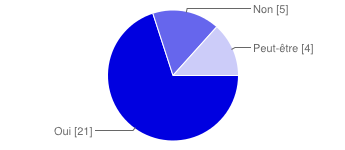
\includegraphics[scale=1.57]{images/chart_1.png}
    \caption{}
    \label{flow}
  \end{center}
\end{figure}

La soirée se déroulera un mercredi soir (18h-23h), serez-vous présent ?

\begin{figure}
  \begin{center}
    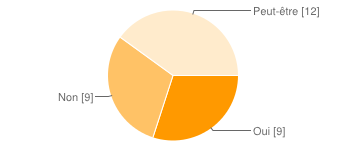
\includegraphics[scale=1.57]{images/chart_2.png}
    \caption{}
    \label{flow}
  \end{center}
\end{figure}

Aimeriez-vous y jouer au cours de cette soirée ?

\begin{figure}
  \begin{center}
    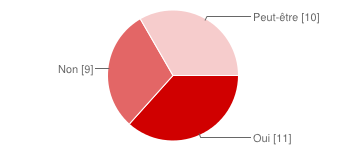
\includegraphics[scale=1.57]{images/chart_3.png}
    \caption{}
    \label{flow}
  \end{center}
\end{figure}

Nous pouvons tirer de ces informations une estimation de plus ou moins 15 personnes présentes si l’on prend
la moitié des \og peut-être \fg{} + les \og oui \fg{}.
En sachant que tous les étudiants ne prêtent pas attention aux mailings de l’université, on peut ajouter
une quinzaine de personnes pour atteindre une estimation de 30 participants.
% subsection l_enquete_d_audience (end)%}}}
\subsection{Les contraintes/ratés}%{{{
\label{sub:les_contraintes_rates}

Un autre moyen de communication fut utilisé, la création d'un évènement
Facebook. Néanmoins cela n'a pas fonctionné, la propagation de cet
évènement ne fut pas suffisante sur le réseau social. De plus cette page
de promotion a été ouverte très tardivement ce qui fait que  nous
n'avons pas eu le temps de faire marcher les connaissances.

La contrainte majeur concernant l'élaboration de la communication fut l'attente
de la confirmation de tous les éléments du projet.  Nous ne pouvions
notamment pas lancer la production des affiches sans savoir si nous
avions un commentateur par exemple.

% subsection les_contraintes_rates (end)%}}}

% section communication (end)%}}}
\section{Bilan financier}%{{{
\label{sec:bilan_financier}

%TODO
Bilan financier
        Prévisionnel
            - salle
            - bar
            - matos
            - intervenant
            - comm
            - repas
        Reel
           ...

% section bilan_financier (end)%}}}
\section{Bilan de la soirée}%{{{
\label{sec:Bilan_de_la_soiree}

\subsection{Prévisionnel}%{{{
\label{sub:previsionnel}

La date de la soirée devait être judicieusement choisie afin d'obtenir une affluence satisfaisante.

Ayant vu grâce au mailing de l’université que la MDE accueillait des soirées chaque jeudi
nommées \og Jeudifférents \fg{}, nous nous sommes dit qu’une soirée comme la notre collait
parfaitement à cette appellation. Malheureusement, nous avions commencé à prendre contact
début février pour la réservation, ce qui fut trop tard. Tous les jeudis sur deux mois étaient
déjà réservés.
Il nous a donc fallu choisir un autre jour de la semaine. Après renseignements auprès de la
MDE, seuls le mercredi et le vendredi étaient libres la semaine du 11 au 17 mars. Le choix ne
fut pas difficile, le mercredi fut choisi naturellement car les étudiants ayant un appartement
dans la métropole rentrent chez eux le vendredi. De plus, le mercredi 13 mars correspondait
au lendemain de la sortie de la nouvelle extension du jeu.
A propos de l’horaire de la soirée, nous avions décidé de commencer dès 18h pour finir à
22h. En effet, le fait de commencer à 18h permet aux étudiants de se rendre à la soirée juste
après les cours. Ensuite, d’après l’AEI, la MDE ferme à 23h et pour ouvrir au-delà de cette
heure, il était nécessaire d’avoir une dérogation pénible à obtenir. Nous nous sommes donc
donné une heure afin d’avoir le temps de remballer, mais également de partir plus tôt pour
reconduire les intervenants chez eux, à Dunkerque.
Après s’être mis d’accord sur la date et l’heure de la soirée, nous devions discuter du
programme.
Il ne fut pas aisé de définir un programme à heures fixes, car les parties n’ont pas une durée
définie. Elles peuvent durer entre 5 et 50 minutes, la moyenne se situant à 25 minutes de jeu.
C’est pourquoi nous avons décidé d’énoncer le contenu de la soirée sans y faire figurer
d’heure.
Nous avions donc prévu de commencer par 20 minutes d’introduction en vidéo sur le jeu et
ses mécanismes afin de pouvoir rendre la soirée plus compréhensible pour les néophytes.
Puis enchainer avec les matchs commentés des intervenants pour finir avec des matchs
confrontant des joueurs du public. Nous avons choisis cet ordre car nous pensions que le plus
amusant était de faire jouer le public, et que cela permettrait de les retenir un maximum.

% subsection previsionnel (end)%}}}
\subsection{Réel}%{{{
\label{sub:reel}

Arrivé le jour J, nous avons été confrontés à plusieurs imprévus.
La météo ne fut pas clémente le 12 mars ainsi que le 13 mars, la neige étant fortement
tombée ces jours là. La circulation était devenue difficile dans la région et beaucoup de cours
furent perturbés.
Ceci impacta fortement l’affluence de la soirée, et surtout son déroulement. Les intervenants
ne purent pas venir du fait des conditions climatiques. Le retour à la fin de la soirée aurait été
dangereux à cause du verglas, et aucun hébergement n’eut pu être possible.
Ces imprévus nous ont donc forcés à improviser.

Les préparatifs commencèrent à 16h, tout se passa bien ou presque. Une fois nos PC personnels
installés, nous nous aperçûmes qu’il fallût utiliser une connectique autre que VGA afin de
connecter nos PC au vidéoprojecteur de la MDE. Heureusement, le directeur de la MDE M.Bross
possédait un vidéoprojecteur VGA avec une bonne qualité de projection.
Une dizaine de personnes arrivèrent passé 18h. Comme prévu à cause du climat, peu de
personnes assistèrent à la soirée. Nous avons recensé une vingtaine de personnes
différentes, mais jamais plus de 11 personnes simultanément.
A cause des imprévus et compte tenu de la faible affluence, nous avons décidé de faire jouer
directement les personnes présentes en projetant leurs parties sur vidéoprojecteur comme
prévu. Julien étant parmi nous le plus expérimenté, il put donc commenter quelques matchs
au cours de la soirée.
Vers 18h50, nous fûmes encore victime d’un imprévu. Les serveurs de jeu de tous les jeux en
ligne de Blizzard tombèrent, nous empêchant de jouer pendant 30 minutes. Pendant ce
temps, nous diffusions les vidéos explicatives de Starcraft II, ce qui permit de combler le
blanc engendré. Néanmoins, un groupe de 4 personnes s’en alla durant ce laps de temps.
Une fois la situation rentrée dans l’ordre, nous pûmes continuer la soirée en petit comité et
terminer à 23h. Entre temps, nous fûmes une pause restauration vers 21h30. Nous
partageâmes les deux plateaux repas en trop avec les participants du fait de l’absence des
deux intervenants. La soirée termina à 23h car nous apprîmes en arrivant pour les préparatifs
que nous pouvions utiliser la salle jusqu’à minuit.
% subsection reel (end)%}}}

% section Bilan_de_la_soiree (end)%}}}


% chapter organisation (end)%}}}
\chapter{Conclusion}%{{{
\label{cha:conclusion}

Au final, bien que la soirée n'amena pas le nombre de participants
escompté, nous sommes heureux que le projet ait pu aboutir.  Jusqu'au
dernier moment nous avons tout fait pour que la soirée puisse avoir
lieu, en trouvant des contournements aux obstacles rencontrés. Par
exemple, la réaction face à l'annulation de la venue des commentateurs.

Bien sûr, nous avons fait des erreurs et la soirée aurait pu mieux être
préparée. Nous aurions dû commencer bien plus tôt notre démarche
concernant la demande de financement auprès de la FSDIE, nous avons donc
été obligés d'avoir recours au budget de la formation pour acheter les
plateaux repas. Cela impliquait également de finir l'organisation de la
soirée pour le début de février, la FSDIE étant stricte à propos de la
constitution du dossier de financement. Nous aurions dû peut-être aussi
accepter l'offre de la team \og aAa \fg{} qui consistait à retransmettre
la soirée sur leur chaine télévisuel en ligne. Peut-être que ça aurait
apporté plus de visibilité à l'évenement sur la scène \og eSportive
\fg{}.

Notre principale erreur était de penser que l'on aurait eu le temps de
tout faire à partir de janvier. En commencant plus tôt, nous aurions pu
faire venir des commentateurs/joueurs plus connus, et surtout commencer
la communication plus tôt même si la soirée n'aurait peut-être pas eu
beaucoup plus de succès à cause des intempéries.


% chapter conclusion (end)%}}}

\appendix

\chapter{Compte rendu 1}%{{{
\label{cha:compte_rendu_1}

\section{Date de la réunion :}
\begin{itemize}
\item La réunion s'est déroulée le vendredi 02 novembre 2012.
\end{itemize}

\section{Objet du jour :}
\begin{itemize}
\item Organisation et analyse du projet de manière générale.
\end{itemize}

\section{Sujets traités :}
\begin{itemize}
\item Le matériel.
\item Le/Les commentateurs.
\item La salle.
\item La publicité.
\end{itemize}

\section{Compte rendu par sujets :}

\subsection{Le matériel}
\begin{itemize}
\item Un ordinateur pour la projection.
\item Un vidéo-projecteur.
\item Un ou plusieurs  micros.
\item Une centaine de chaises.
\end{itemize}

\subsection{Le/Les commentateurs}
\begin{itemize}
\item Il nous faut au minimum 1 commentateur, il serait intéressant d'en avoir plusieurs.
\item Si nous n'arrivons pas à trouver de commentateurs ni de joueurs, Julien se propose pour faire une démonstration étant donné que c'est un joueur de SC2. Dans le pire des cas, faire jouer des participants.
\end{itemize}

\subsection{La salle}
\begin{itemize}
\item Nous avons décidé d'emprunter la maison de l'étudiant un soir de la semaine, de préférence un jeudi (jour de bière autorisé!).
\end{itemize}

\subsection{La publicité}
\begin{itemize}
\item Des affiches / flyers.
\item Liste de diffusion des étudiants de Lille 1.
\item Sites communautaires d' \og e-sport \fg{} français.
\end{itemize}

\section{La répartition du travail}

\subsubsection{Jean-François:}
\begin{itemize}
\item Réalisation de l'affiche / flyers.
\item Contacter des sites communautres pour la communication.
\end{itemize}

\subsubsection{Julien :}
\begin{itemize}
\item Contacter des équipes françaises d'e-sport.
\item Contacter la FNAC pour de la publicité.
\item Contacter Blizzard pour éventuellement avoir de la décoration.
\end{itemize}

\subsubsection{Yannick :}
\begin{itemize}
\item Contacter l'équipe de l'illico pour la communication par e-mail.
\item Contacter l'imprimerie de Lille1 pour l'impression de l'affiche et des flyers.
\end{itemize}


% chapter  (end)%}}}
\chapter{Compte rendu 2}%{{{
\label{cha:compte_rendu_2}

\section{Date de la réunion :}
\begin{itemize}
\item La réunion s'est déroulée le vendredi 14 décembre 2012.
\end{itemize}

\section{Objet du jour :}
\begin{itemize}
\item Apporter des précisions et discuter des premiers avancements.
\end{itemize}

\section{Sujets traités :}
\begin{itemize}
\item Le nom de la soirée.
\item Le financement.
\item La programmation de la soirée.
\item La répartition du travail.
\end{itemize}

\section{Compte rendu par sujet :}

\subsection{Le nom de la soirée}
\begin{itemize}
\item Le nom de la soirée : Barcraft of Legends (susceptible de changer).
\end{itemize}

\subsection{Le financement :}
\begin{itemize}
\item Après réponse des sponsors, ils ne veulent pas financer l’événement car ils considèrent que c'est une prestation de service.  Nous allons donc démarcher d'autres équipes en attendant notre demande de financement et des amateurs qui souhaitent se lancer dans le commentaires de matchs ou showmatch.
\item Le coût est évalué à environ 500 euros pour déplacer 2 joueurs et 1 commentateur (1 sur Lille).
\end{itemize}

\subsection{La programmation de la soirée}
\begin{itemize}
\item Dans tout les cas, l'équipe aAa propose de faire une diffusion en direct (streaming) sur leur site (à voir avec la connexion).
\end{itemize}

\section{La répartition du travail :}

\subsubsection{Jean-François :}
\begin{itemize}
\item Réalisation de l'affiche / flyers (en cours).
\item Voir avec l'imprimerie de Lille 1.
\end{itemize}

\subsubsection{Julien :}
\begin{itemize}
\item Contacter des commentateurs amateurs ou professionnels.
\item Contacter la FNAC pour de la publicité.
\item Contacter blizzard pour éventuellement avoir de la décoration.
\item Prise de rendez-vous avec le manager aAa qui est sur Lille.
\end{itemize}

\subsubsection{Yannick :}
\begin{itemize}
\item Envoi des mails aux différentes associations.
\item Constitution du dossier de demande de financement (FSDIE).
\item Contacter \og Des A La Carte \fg{} et l'AEI\footnote{L'Association des Étudiants en Informatique.} qui ont l'habitude d'organiser ce genre d’événement.
\end{itemize}


% chapter  (end)%}}}
\chapter{Compte rendu 3}%{{{
\label{cha:compte_rendu_3}

\section{Date de la réunion :}
\begin{itemize}
\item La réunion s'est déroulée le vendredi 14 décembre 2012.
\end{itemize}

\section{Objet du jour :}
\begin{itemize}
\item Apporter des précisions et discuter des premiers avancements.
\end{itemize}

\section{Sujets traités :}
\begin{itemize}
\item Le nom de la soirée.
\item Le financement.
\item La programmation de la soirée.
\item La répartition du travail.
\end{itemize}

\section{Compte rendu par sujet :}

\subsection{Le nom de la soirée}
\begin{itemize}
\item Le nom de la soirée : Barcraft of Legends (susceptible de changer).
\end{itemize}

\subsection{Le financement :}
\begin{itemize}
\item Après réponse des sponsors, ils ne veulent pas financer l’événement car ils considèrent que c'est une prestation de service.  Nous allons donc démarcher d'autres équipes en attendant notre demande de financement et des amateurs qui souhaitent se lancer dans le commentaires de matchs ou showmatch.
\item Le coût est évalué à environ 500 euros pour déplacer 2 joueurs et 1 commentateur (1 sur Lille).
\end{itemize}

\subsection{La programmation de la soirée}
\begin{itemize}
\item Dans tout les cas, l'équipe aAa propose de faire une diffusion en direct (streaming) sur leur site (à voir avec la connexion).
\end{itemize}

\section{La répartition du travail :}

\subsubsection{Jean-François :}
\begin{itemize}
\item Réalisation de l'affiche / flyers (en cours).
\item Voir avec l'imprimerie de Lille1.
\end{itemize}

\subsubsection{Julien :}
\begin{itemize}
\item Contacter des commentateurs amateurs ou professionnels.
\item Contacter la FNAC pour de la publicité.
\item Contacter blizzard pour éventuellement avoir de la décoration.
\item Prise de rendez-vous avec le manager aAa qui est sur Lille.
\end{itemize}

\subsubsection{Yannick :}
\begin{itemize}
\item Envoi des mails au différentes associations.
\item Constitution du dossier de demande de financement (FSDIE).
\item Contacter \og Des A La Carte \fg{} et l'AEI\footnote{L'Association des Étudiants en Informatique.} qui ont l'habitude d'organiser ce genre d’événement.
\end{itemize}


% chapter  (end)%}}}
\chapter{Compte rendu 4}%{{{
\label{cha:compte_rendu_4}

\section{Date de la réunion:}
\begin{itemize}
\item La réunion s'est déroulée le vendredi 21 décembre 2012
\end{itemize}

\section{Objet du jour:}
\begin{itemize}
\item Problèmes inhérents au réseau de la cité scientifique
\end{itemize}

\section{Sujets traités:}
\begin{itemize}
\item Le réseau
\item Le financement
\item La répartition du travail
\item La communication autour de la formation
\end{itemize}

\section{Compte rendu par sujet:}

\subsection{La communication autour de la formation:}
\begin{itemize}
\item Le logo de la formation
\item Les plaquettes décrivant la formation

\end{itemize}

\subsection{Le financement:}
\begin{itemize}
\item Finalement, le coût en déplacement va être supérieur à 500 euros
puisque la personne qui est sur Lille va déménager prochainement. Nous
avons décidé de limité le nombre de personnes venant de l'extérieur.
\end{itemize}

\subsection{Connexion:}
\begin{itemize}
\item Pour les problèmes de proxy, nous en avons discuté avec M.Mathieu. En effet, les ports attribués pour les jeux-vidéos ne passent pas à travers le proxy de la cité scientifique. De ce fait, nous ne pouvions pas définir précisément le contenu de la soirée sans régler ce problème. D'après M.Mathieu, les changements de paramètres du proxy se font assez facilement que ça soit pour la durée de déblocage ou le temps de déblocage des ports
\end{itemize}

\section{Répartition du travail:}

\subsubsection{Jean-François:}
\begin{itemize}
\item Réalisation de l'affiche / flyers
\item Voir avec l'imprimerie de Lille1
\end{itemize}

\subsubsection{Julien:}
\begin{itemize}
\item Contacter des commentateurs amateurs ou professionnels
\item Contacter la FNAC pour de la publicité
\item Contacter blizzard pour éventuellement avoir de la décoration
\item Prise de rendez-vous avec le manager aAa qui est sur Lille
\end{itemize}

\subsubsection{Yannick:}
\begin{itemize}
\item Envoi des mails au différentes associations
\item Constitution du dossier de demande de financement (FSDIE)
\item Contacter \og Des À La Carte \fg{} et l'AEI\footnote{L'Association des Étudiants en Informatique.} qui sont des associations qui ont l'habitude d'organiser ce genre d’événement
\end{itemize}


% chapter  (end)%}}}

\end{document}%}}}
